\documentclass[a4paper, titlepage]{article}

\usepackage[round, sort, numbers]{natbib}
\usepackage[utf8]{inputenc}
\usepackage{amsfonts, amsmath, amssymb, amsthm}
\usepackage{blkarray}
\usepackage{color}
\usepackage{mathtools}
\usepackage{paralist}
\usepackage{parskip}
\usepackage{subcaption}
\usepackage{tikz}
\usepackage{titlesec}

\numberwithin{figure}{section}
\numberwithin{table}{section}

\usetikzlibrary{arrows, automata, backgrounds, petri, positioning}
\tikzstyle{place}=[circle, draw=blue!50, fill=blue!20, thick]
\tikzstyle{marking}=[circle, draw=blue!50, thick, align=center]
\tikzstyle{transition}=[rectangle, draw=black!50, fill=black!20, thick]

% define new commands for sets and tuple
\newcommand{\setof}[1]{\ensuremath{\left \{ #1 \right \}}}
\newcommand{\tuple}[1]{\ensuremath{\left \langle #1 \right \rangle }}
\newcommand{\card}[1]{\ensuremath{\left \vert #1 \right \vert }}

\makeatletter
\newcommand\objective[1]{\def\@objective{#1}}
\newcommand{\makecustomtitle}{%
	\begin{center}
		\huge\@title \\
		[1ex]\small Dimitri Racordon
	\end{center}
	\@objective
}
\makeatother

\begin{document}

\title{Outils formels de Modélisation \\ 9\textsuperscript{ème} séance d'exercices}
\author{Dimitri Racordon}
\objective{
Dans cette séance d'exercices, nous allons poursuivre notre étude de l'algèbre linéaire dans le cadre des réseaux de Petri en utilisant les P/T-invariants.
}

\makecustomtitle

\section{Producteur/consommateur ($\bigstar\bigstar$)}
Considérez le réseau de la figure \ref{fig:robots-model}, lequel représente un modèle \emph{producteur consommateur}.
Sa matrice d'incidence est décrite par la figure \ref{fig:robots-incidence}.

\begin{figure}[ht]
	\centering
  \begin{minipage}[b]{.48\linewidth}
  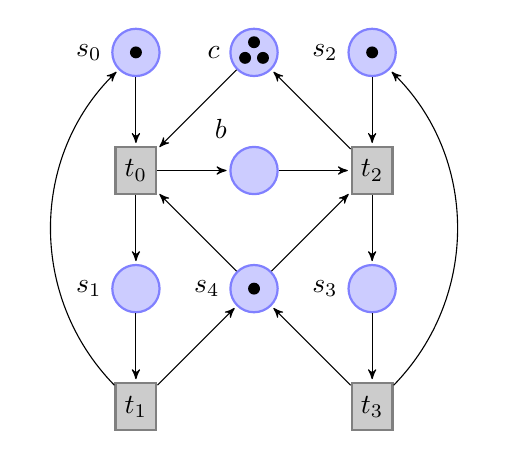
\begin{tikzpicture}[node distance=1.5cm, minimum height=6mm, >=stealth', bend angle=45, auto]
    \node[place,tokens=1] (s0) [label=left:$s_0$] {};
    \node[place] (s1) [below of=s0, yshift=-1.5cm, label=left:$s_1$] {};

    \node[place,tokens=3] (cb) [right of=s0, label=left:$c$] {};
    \node[place] (b) [below of=cb, label=135:$b$] {};
    \node[place,tokens=1] (s4) [below of=b, label=left:$s_4$] {};

    \node[place,tokens=1] (s2) [right of=cb, label=left:$s_2$] {};
    \node[place] (s3) [below of=s2, yshift=-1.5cm, label=left:$s_3$] {};

    \node [transition] (t0) [below of=s0] {$t_0$}
				  edge [pre] (s0) edge [pre] (cb) edge [pre] (s4)
          edge [post] (b) edge [post] (s1);
    \node [transition] (t1) [below of=s1] {$t_1$}
				  edge [pre] (s1)
          edge [post,bend left] (s0) edge [post] (s4);

    \node [transition] (t2) [below of=s2] {$t_2$}
				  edge [pre] (s2) edge [pre] (s4) edge [pre] (b)
          edge [post] (cb) edge [post] (s3);
    \node [transition] (t3) [below of=s3] {$t_3$}
				  edge [pre] (s3)
          edge [post,bend right] (s2) edge [post] (s4);
  \end{tikzpicture}
  \subcaption{Réseau de Petri}
  \label{fig:robots-model}
  \end{minipage}
  \hfill
  \begin{minipage}[b]{.48\linewidth}
  \[
  \begin{blockarray}{rrrrr}
  & t_0 & t_1 & t_2 & t_3 \\
  \begin{block}{c(rrrr)}
    s_0 & -1 &  1 &  0 &  0 \\
    s_1 &  1 & -1 &  0 &  0 \\
    s_2 &  0 &  0 & -1 &  1 \\
    s_3 &  0 &  0 &  1 & -1 \\
    s_4 & -1 &  1 & -1 &  1 \\
    b   &  1 &  0 & -1 &  0 \\
    c   & -1 &  0 &  1 &  0 \\
  \end{block}
  \end{blockarray}
  \]
  \subcaption{Matrice d'incidence}
  \label{fig:robots-incidence}
  \end{minipage}
\end{figure}

En appliquant l'algorithme de Farkas:
\begin{enumerate}
  \item Déterminez les P-invariants de ce réseau.
  \item Déterminez les T-invariants de ce réseau.
\end{enumerate}
Puis:
\begin{enumerate}
  \setcounter{enumi}{2}
  \item Vérifiez que les invariants que vous avez calculés sont correctes à l'aide d'un outil de calcul de votre choix.
\end{enumerate}

Vous pouvez vous servir du code Swift fourni en annexe, lequel propose une modeste bibliothèque pour manipuler des matrices.

\section{Preuve de non-bloquage ($\bigstar\bigstar\bigstar$)}

A l'aide des invariants que vous avez calculez dans l'exercice précédent, prouvez que le réseau de la figure \ref{fig:robots-model} ne peut pas être bloqué.

\end{document}
